\documentclass[tikz, border=10pt]{standalone}
\usepackage{tikz}
\usetikzlibrary{shapes, positioning, arrows.meta, calc}

\begin{document}
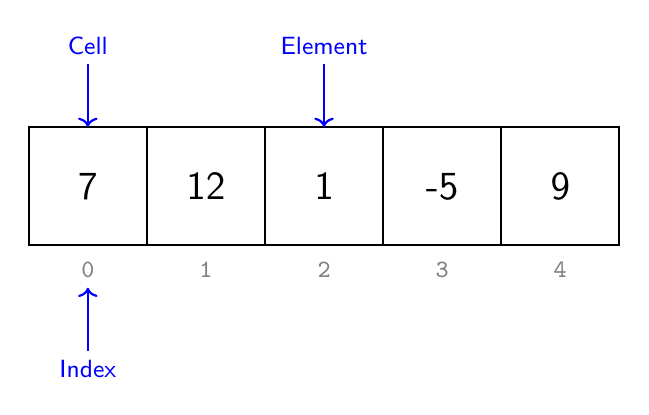
\begin{tikzpicture}[
    cell/.style={
        rectangle, 
        draw=black, 
        thick, 
        minimum width=1.5cm, 
        minimum height=1.5cm, 
        node distance=0cm, 
        outer sep=0pt,
        font=\Large\sffamily
    },
    label_text/.style={
        font=\sffamily\small\color{blue}
    }
]

    % Array cells
    \node[cell] (c0) {7};
    \node[cell, right=of c0] (c1) {12};
    \node[cell, right=of c1] (c2) {1};
    \node[cell, right=of c2] (c3) {-5};
    \node[cell, right=of c3] (c4) {9};

    % Indices
    \node[below=0.1cm of c0, font=\small\ttfamily\color{gray}] (idx0) {0};
    \node[below=0.1cm of c1, font=\small\ttfamily\color{gray}] (idx1) {1};
    \node[below=0.1cm of c2, font=\small\ttfamily\color{gray}] (idx2) {2};
    \node[below=0.1cm of c3, font=\small\ttfamily\color{gray}] (idx3) {3};
    \node[below=0.1cm of c4, font=\small\ttfamily\color{gray}] (idx4) {4};

    % Annotations
    % Cell
    \node[above=0.8cm of c0, label_text] (lbl_cell) {Cell};
    \draw[->, blue, thick] (lbl_cell) -- (c0.north);

    % Element
    \node[above=0.8cm of c2, label_text] (lbl_elem) {Element};
    \draw[->, blue, thick] (lbl_elem) -- (c2.north);

    % Index
    \node[below=0.8cm of idx0, label_text] (lbl_idx) {Index};
    \draw[->, blue, thick] (lbl_idx) -- (idx0.south);

\end{tikzpicture}
\end{document}
